\chapter{Umsetzung}
\section{Das OSGi Framework}
%\begin{wrapfigure}{r}{9.0cm}
%	\begin{center}
%		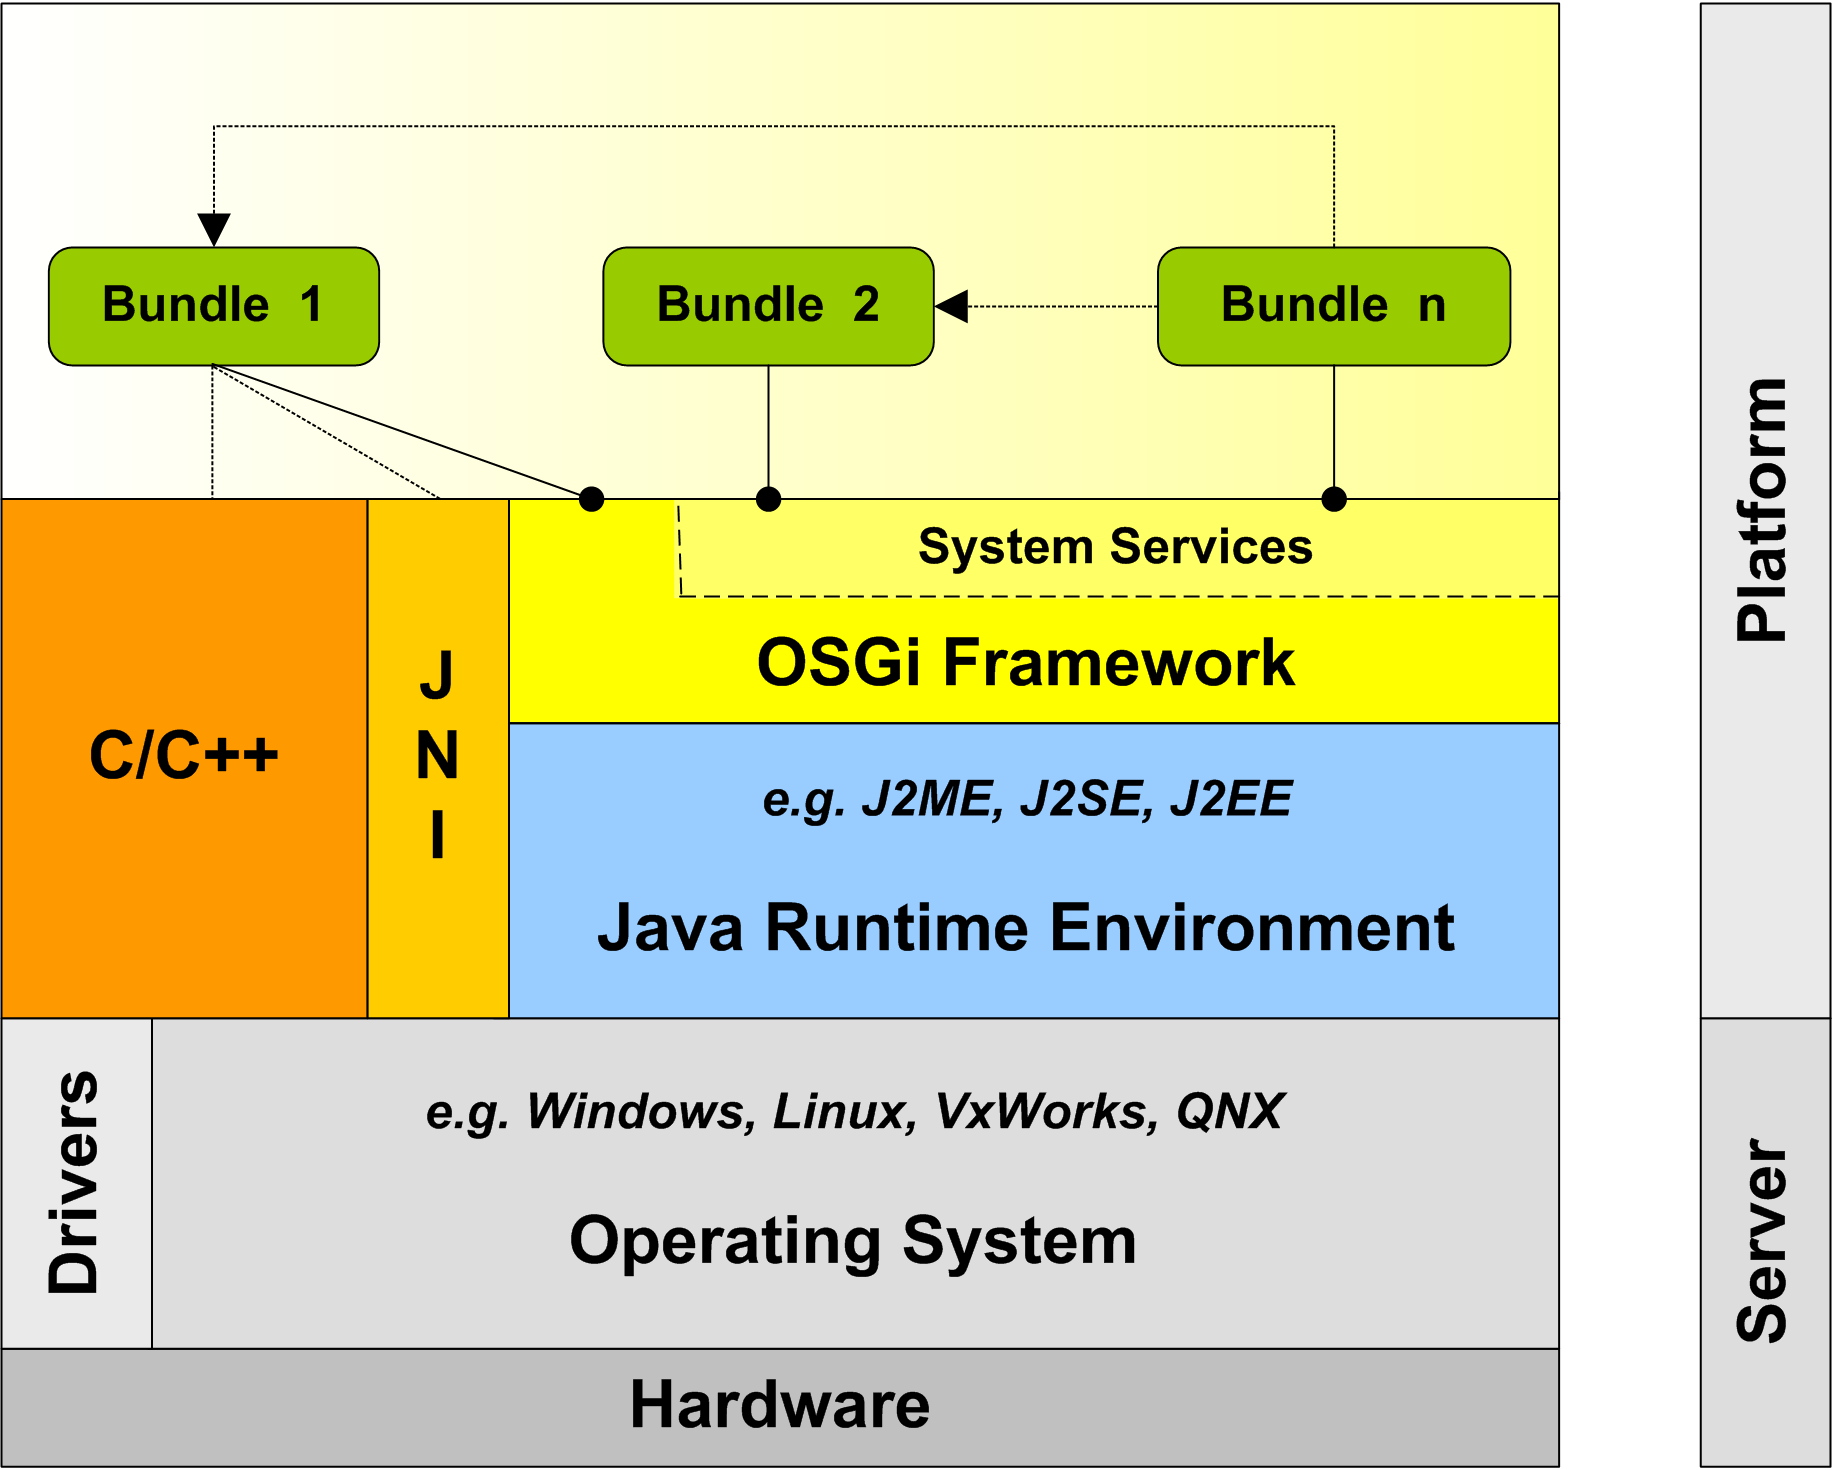
\includegraphics[width=8.5cm]{pics/osgi_layer.png}
%	\caption{something, citing}
%	\end{center}
%	\label{fig:hmm}
%\end{wrapfigure}
Die \textbf{OSGi Alliance}, früher
\enquote{\textit{Open Services Gateway initiative}}, ist ein Zusammenschluß
verschiedener Unternehmen, wie z.B. IBM, Oracle oder Sun Microsystems.
\index{OSGi Alliance}
\index{OSGi|see{OSGi Alliance}}
\index{Open Services Gateway|see{OSGi Alliance}}
Sie spezifiziert die \textbf{OSGi Service Platform}, ein Java-basiertes
Application-Framework, mit dessen Hilfe modulare, service-orientierte
Anwendungen erstellt werden können. Einzelne Module, sogenannte
\textbf{Bundles}, können der Anwendung dynamisch hinzugefügt und wieder
entfernt werden. Ein erneutes Kompilieren oder Starten der Anwendung ist dazu
nicht erforderlich.
\index{OSGi Service Platform}
\index{Bundle}
Das Framework bietet ausserdem eine globale \textbf{Service Registry}, an der
Bundles sogenannte \textbf{Services} anmelden und abgefragen können.
% OSGi Framework = OSGi Service Platform without OSGi Standard Services 13
\citep{wtherich_die_2008}
\index{Service Registry}
\index{Service}

\begin{figure}[p]
	\begin{center}
		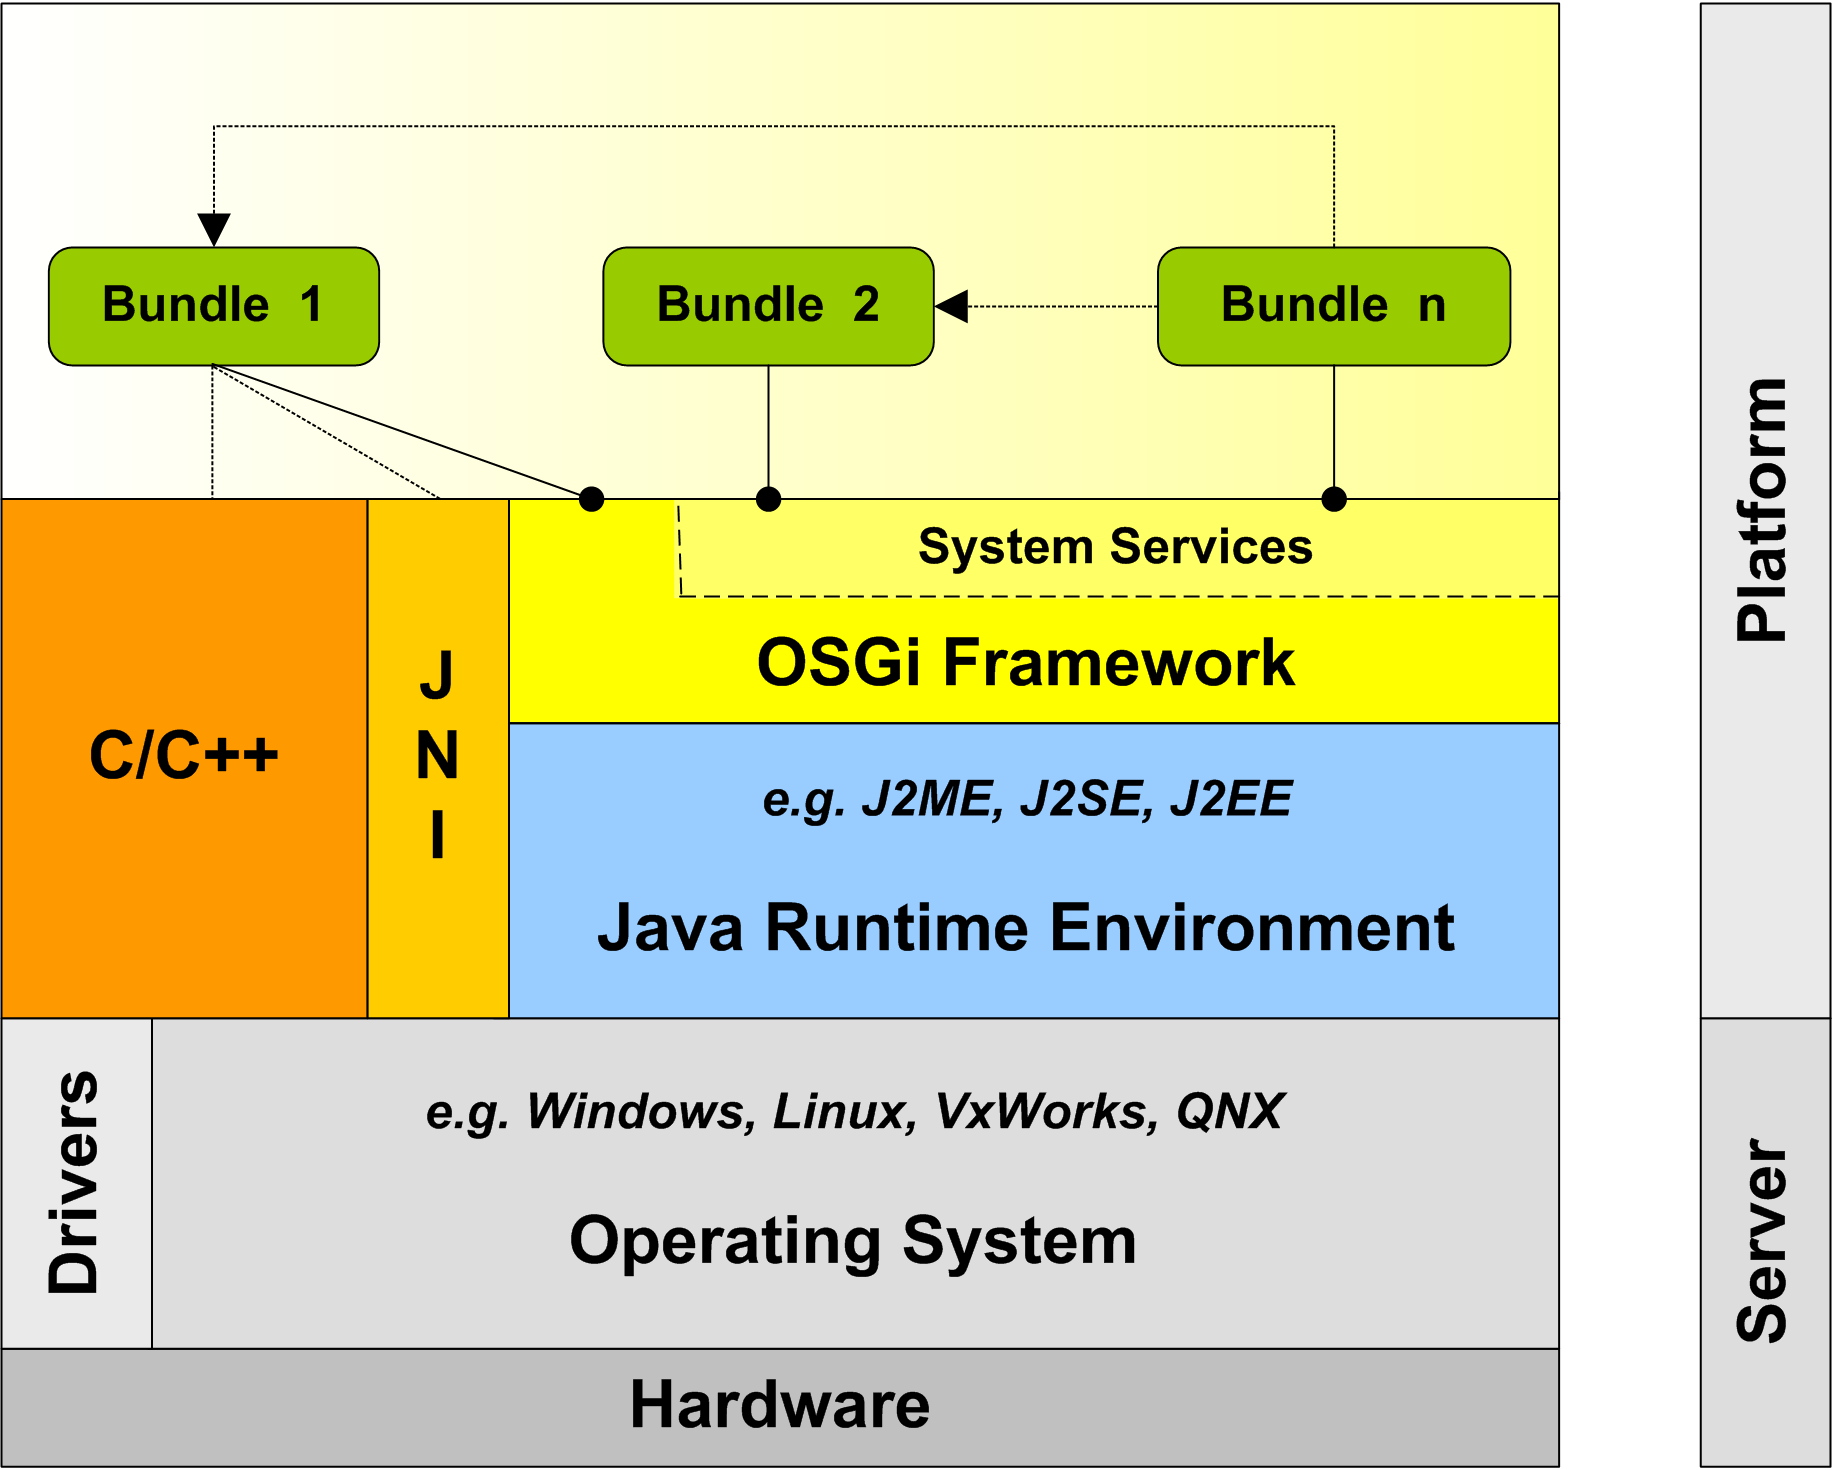
\includegraphics[scale=2]{pics/osgi_layer.png}
	\caption[OSGi layers]{
	\textbf{OSGi layers.}
	something}
	\end{center}
	\label{fig:osgi_layer}
\end{figure}

\subsection{Bundles}
Ein Bundle stellt technisch eine Einheit von Klassen und Ressourcen dar, die
eigentständig in der Anwenung gestartet, gestoppt, installiert und
deinstalliert werden können.
\citep{wtherich_die_2008}
% selbe version 17
% importieren, exportieren 13,79
% class loading 89
% MANIFEST.MF 21
% lebenszyklen 23,55
% unterschied Bundle / Plug-In 41

\subsection{Services} % 93
Ein Service ist ein Java-Object, typischerweise ein Interface, das unter dem
Interface-Namen an der Service Registry angemeldet wird.
\index{Service Registry}
Die Service Registry steht bundleübergreifend in der Anwendung zu Verfügung.
Wird ein bestimmer Dienst von einem Bundle benötigt, kann dieser an der Service
Registry abgefragt werden, ohne dass im Enzelnen bekannt sein muss, welche
Implementierung dahinter steckt oder welches Bundle diesen Dienst anbietet.
\index{Bundle}
% Services können kommen und gehen 23
% Standard Services 13,25
\citep{wtherich_die_2008}
\section{Anna}
Die Basis der Pipeline bildet das OSGi Framework, sowie
eine Auswahl an Standard-Services.
\index{Pipeline}
\index{OSGi Framework}
\index{Standard-Services}
Folgende Bundles aus der OSGi Service Plattform werden zur Ausführung der
Pipeline benötigt:
\begin{itemize}
  \item
  \begin{verbatim}org.eclipse.osgi_3.4.0.v20080605-1900.jar\end{verbatim}
  \item
  \begin{verbatim}org.eclipse.equinox.common_3.4.0.v20080421-2006.jar\end{verbatim}
  \item
  \begin{verbatim}org.eclipse.equinox.log_1.1.0.v20080414.jar\end{verbatim}
  \item
  \begin{verbatim}org.eclipse.equinox.util_1.0.0.v20080414.jar\end{verbatim}
  \item
  \begin{verbatim}org.eclipse.osgi.services_3.1.200.v20071203.jar\end{verbatim}
  \item
  \begin{verbatim}org.eclipse.osgi.util_3.1.300.v20080303.jar\end{verbatim}
\end{itemize}

\begin{figure}[ht]
	\begin{center}
		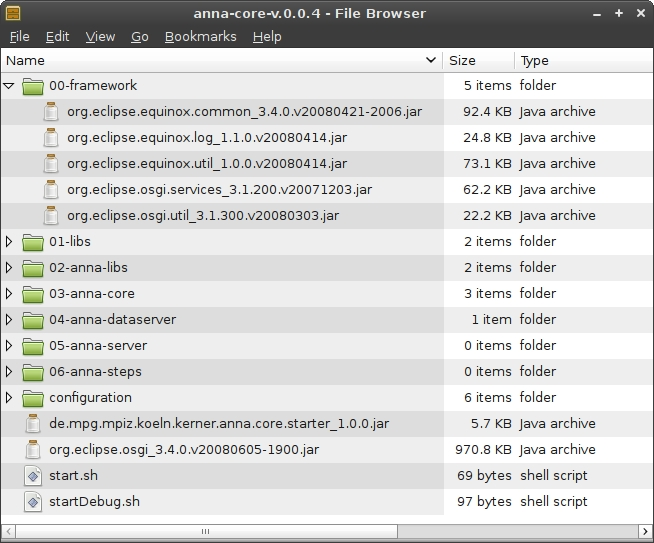
\includegraphics[scale=0.68]{pics/anna_folder_framework.jpg}
	\caption[Application core]{
	\textbf{Application core.}
	something}
	\end{center}
	\label{fig:anna_folder_framework}
\end{figure}

Über die Konfigurationsdatei des OSGi Frameworks ist festgelegt, dass beim
Starten des Frameworks das Bundle
\begin{verbatim}de.mpg.mpiz.koeln.anna.core.starter_1.0.0.jar\end{verbatim}
automatisch installiert und gestartet wird. Dieses Bundle initialisiert und
startet die Pipeline, indem es alle Bundles, die sich in den Unterverzeichnissen
\texttt{00-*} bis \texttt{06-*} des working directories befinden, installiert
und startet. Die Verzeichnisse \texttt{00-*} bis \texttt{03-*} enthalten
hierbei Bundles, die gewisse Kernfunktionalitäten bereitstellen, wie z.B. die
benötigten OSGi Standard-Services oder andere Biblioteken, wie z.B.
\texttt{bioutils} oder \texttt{kerner-commons}.
Die Verzeichnisse \texttt{04-*} und \texttt{05-*} enhalten den
Pipeline-Server, Verzeichnis \texttt{06-*} soll alle Bundles enthalten, die
einen Pipeline Step zur Verfügung stellen.
Die Verzeichnisse werden nach ihrer numerischen Reihenfolge abgearbeitet.
Angefangen bei Verzeichnis \texttt{00-*} bis zu Verzeichnis \texttt{06-*} werden
alle im jeweiligen Verzeichnis vorhandene Bundles installiert und im direkten
Anschluss gestartet. Unterverzeichnisse werden nicht berücksichtigt.

\subsection{Server}
Der Pipeline Server besteht aus zwei Elementen: Zum einen einem 
Step Executor, der die einzelnen Steps zur Ausführung bringt, sowie einen
Data Proxy, der den Zugriff auf das \code{DataBean} Objekt steuert.
Step Executor sowie Data Proxy sind als OSGi Service implementiert.
\code{AbstractStep} implementiert \code{BundleActivator}, so dass er den
Pipeline Server Service an der \textit{Service Registry} abfragen und sich dort
registrieren kann.
\index{Server|see{Pipeline-Server}}
\index{Pipeline-Server}
\index{Data Proxy}
\index{OSGi Service}
\index{DataBean}
%\lstinputlisting[frame=single,label=server,caption=Application
%Server]{code/server}

\subsubsection{StepExecutor}
Wird ein Step am Server registriert, wird er an einen StepExecutor übergeben,
der die Ausführung des Steps überwacht und steuert. Er ruft im wesentlichen
die drei Callback Methoden von \code{Step} auf.
\lstinputlisting[frame=single,label=step,caption=Step]{code/step}

\subsubsection{DataProxy}
Die Pipeline persistiert die (Zwischen-)Ergebnisse einzelner Steps, um bei
einer gewollten oder ungewollten Unterbrechung des Programms die bis dahin
gewonnenen Daten nicht zu verlieren. Eine \code{Step} Implementierung bekommt
beim Aufruf der Callback Methoden eine Refrenz auf einen Data Proxy, über den
die aktuell in der Pipeline verfügbaren Daten abgefragt werden können. Der
Proxy kontrolliert den Zugriff auf die Daten und implementiert dabei alle
Aspekte der Synchronization und Serialisierung der Daten.

\begin{figure}[ht]
	\begin{center}
		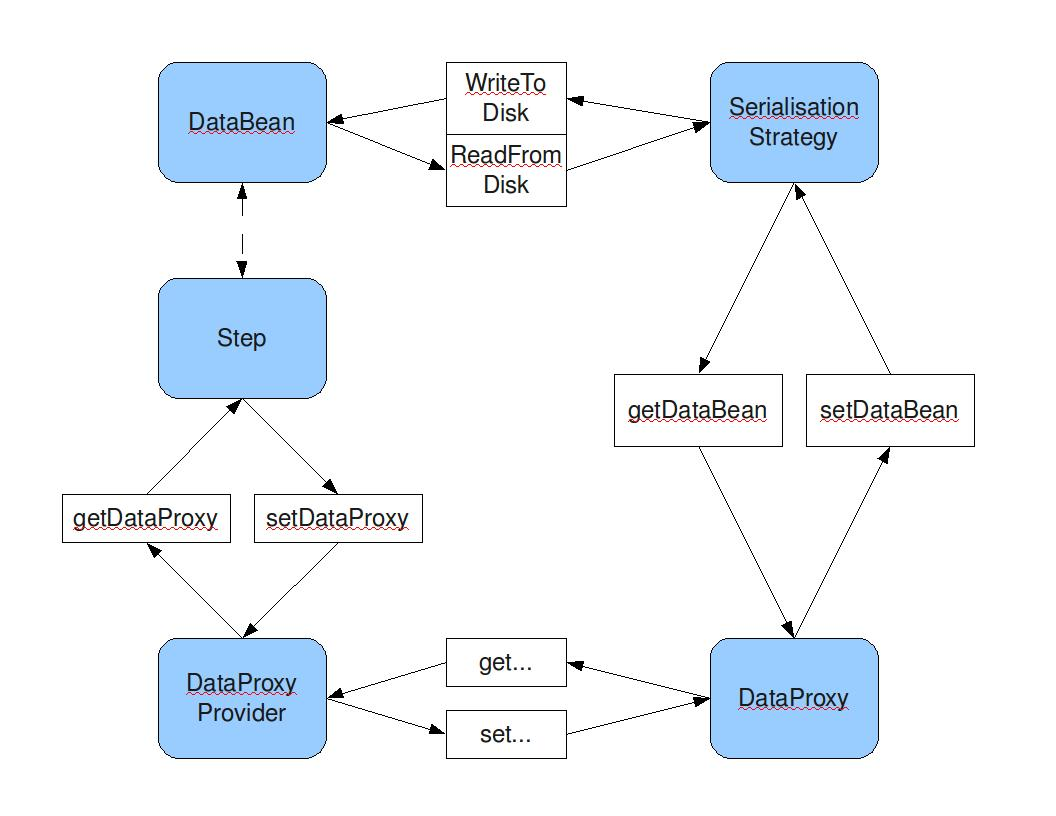
\includegraphics[scale=0.42]{pics/programDataManagment.jpg}
	\caption[Data Management]{
	\textbf{Data Management.}
	something}
	\end{center}
	\label{fig:programDataManagment}
\end{figure}

\subsection{Steps}
Ein Pipeline Step muss von \code{AbstractStep} erben.
\subsubsection{Conrad}
Conrad
(\htmladdnormallink{http://www.broadinstitute.org/annotation/conrad/}{http://www.broadinstitute.org/annotation/conrad/})
ist ein \textit{de novo} gene caller, der Genstrukturen wie Exons und Introns
vorhersagen kann.
\index{Conrad} \index{de novo}\index{gene caller}
Die Vorhersage stützt sich dabei auf \textit{semi-Markow Conditional Random
Fields}, kurz \textbf{CRF}.  % wird in hintergründen erwähnt
\index{Markow} \index{Conditional Random Fields} \index{CRF|see{Conditional
Random Fields}}
Conrad benötigt für seine Genvorhersage eine FASTA-Datei mit einer oder
mehreren zu analysierenden DNA-Sequenzen, sowie eine Binärdatei, die Parameter
für den CRF-Alorithmus entält.
Diese Binärdatei wird in einem Trainingslauf erstellt, der vor der
eigentlichen Genvorhersage durchgeführt wird. Hierbei wird der CRF-Algorithmus
auf die Eingabesequenz trainiert, um die Qualität der Genvorhersage
zu maximieren. Dieser Trainingslauf benötigt eine FASTA-Datei mit
DNA-Sequenzen, die Gene enthalten, sowie eine GFF-Datei mit Annotationen zu
diesen Genen.
Die DNA-Sequenzen, die für das Training herangezogen werden, bestimmen direkt
die Qualität der späteren Genvorhersage:
Je \enquote{ähnlicher} die Trainingssequenzen den Sequenzen für die
Vorhersage sind, desto genauer wird das Ergebnis.
\citep{doherty_gene_2007}

Um einen Eindruck von der Qualität der Genvorhersage zu gewinnen, wurden
mehrere Trainings- und Vorhersage-Schritte mit einem Beispieldatensatz aus dem
Conrad-Packet durchgeführt, deren Ergebnisse dann kreuzvalidiert wurden.
Der Beispieldatensatz beinhaltete 574 Sequenzen von \texttt{Aspergillus niger},
die dazu im Verhältnis 1:10 in zwei Datensätze \enquote{testing} und
\enquote{training} aufgeteilt wurden. Das Training erfolgte mit dem
\enquote{training}-Datensatz, die anschliessende Vorhersage wurde für beide
Datensätze durchgeführt.
\index{Aspergillus niger}

Das Ergebnis hieraus war also zum einen eine Vorhersage für eben die Sequenzen,
mit denen Conrad zuvor trainiert wurde, zum Anderen eine Vorhersage für unbekannte
Sequenzen, welcher allerdings ein optimales Training vorrausgegangen war.

Das Ergebnis der Genvorhersage für die beiden Datensätze \enquote{training} und
\enquote{testing} stellt sich wie folgt dar:\\
Die Werte für den \enquote{training}-Datensatz sind generell relativ konstant,
für den \enquote{testing}-Datensatz sind sie weiter gestreut.
Diese Verteilung ist zu erwarten und zeigt ein ausgewogenes Training.
Das bei einem Training oft auftretende \textit{over fitting} ist nicht
festzustellen.
\index{over fitting}
Die Qualität der Genvorhersagen stellt sich in sechs Kategorien dar:
\begin{description}
\item[prediction sensitivity for coding exons] ist das Verhältnis
der gefundenen Exons zu den tatsächlichen vorhandenen Exons.
\item[prediction specificity for coding exons] \ldots
\item[prediction sensitivity for coding nucleotides] \ldots
\item[prediction specificity for coding nucleotides] \ldots
\item[perfectly predicted sequences] ist das Verhältnis aller
vollständig korrekt vorhergesagten Exons zu der Gesamtmenge an Exons.
\item[nucleotide hidden state agreement] ist das Verhältnis der vorhergesagten
Basen-\enquote{Zustände} zu den tatsächlichen Basen-Zuständen.
\end{description}

\begin{figure}[ht]
	\begin{center}
		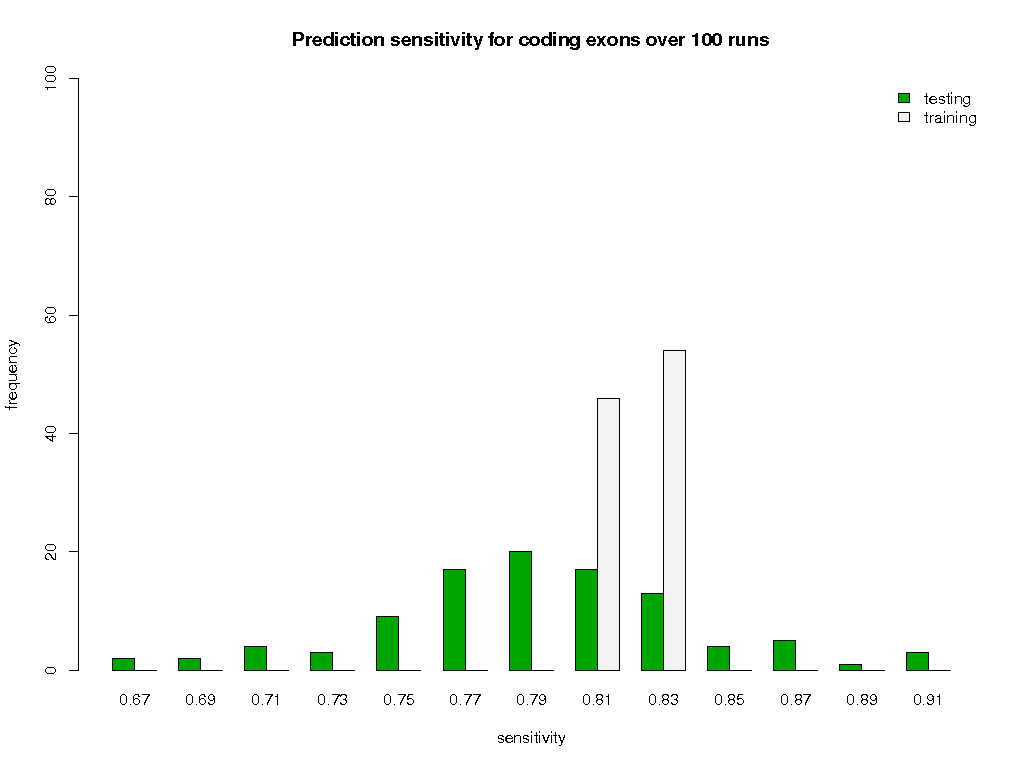
\includegraphics[scale=0.42]{pics/codingExons_sens.png}
	\caption[Prediction sensitivity for coding exons over 100 runs]{
	\textbf{Prediction sensitivity for coding exons over 100 runs.}
	something}
	\end{center}
	\label{fig:codingExons_sens}
\end{figure}

\begin{figure}[ht]
	\begin{center}
		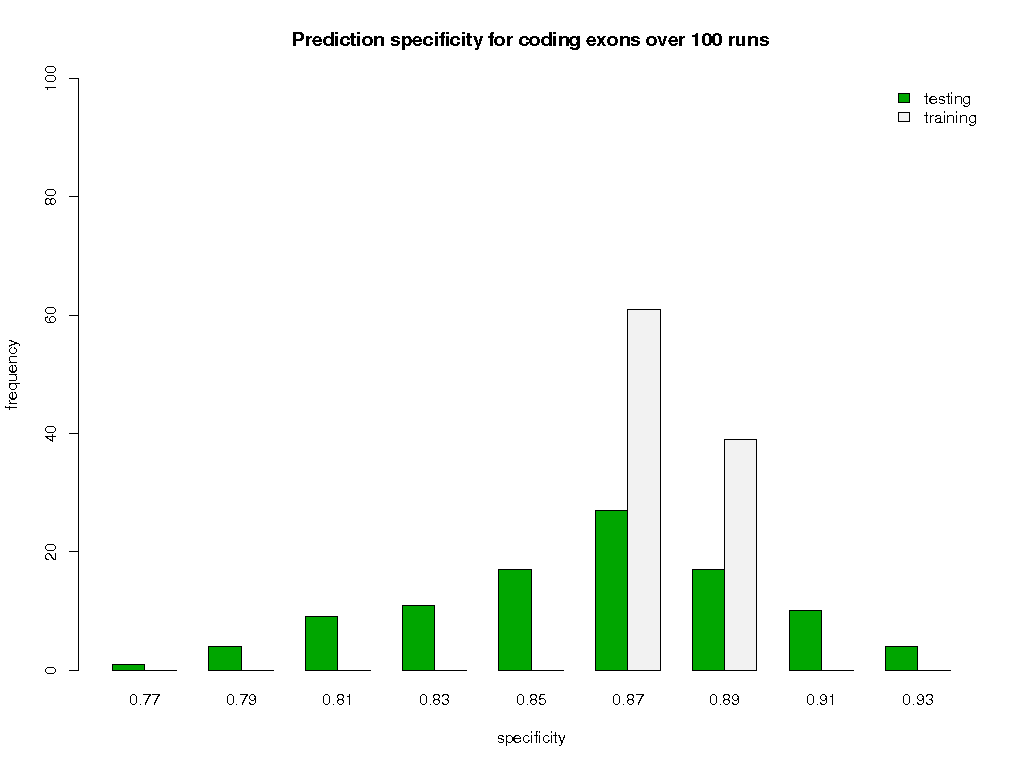
\includegraphics[scale=0.42]{pics/codingExons_spec.png}
	\caption[Prediction specificity for coding exons over 100 runs]{
	\textbf{Prediction specificity for coding exons over 100 runs.}
	something}
	\end{center}
	\label{fig:codingExons_spec}
\end{figure}

\begin{figure}[ht]
	\begin{center}
		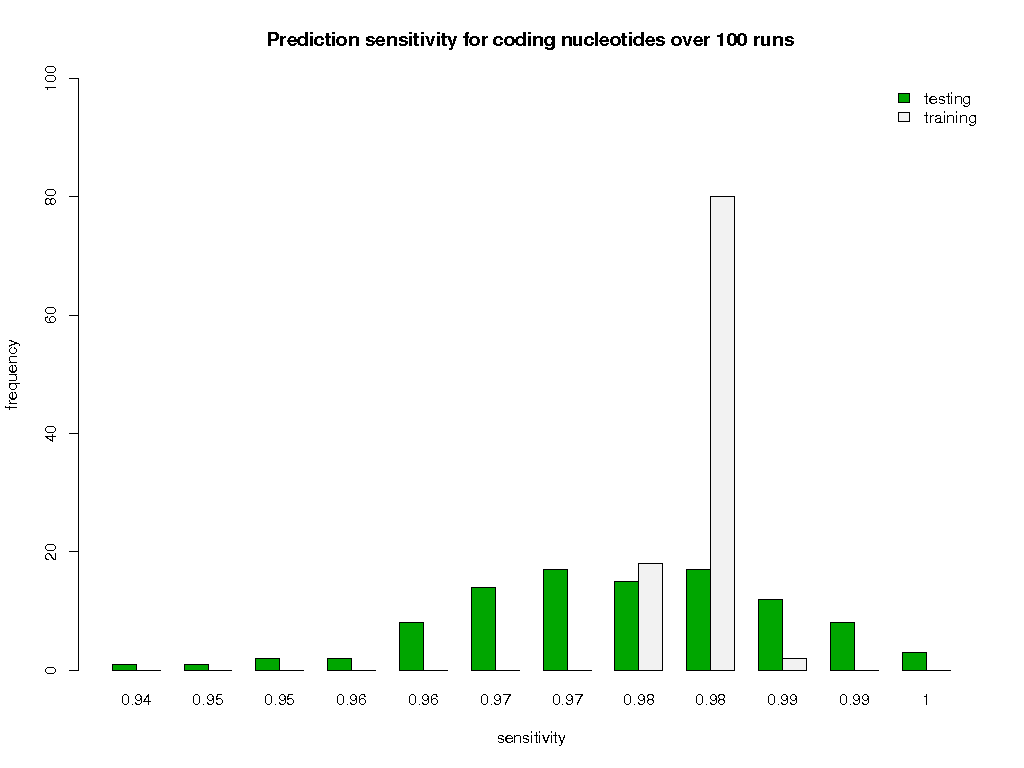
\includegraphics[scale=0.42]{pics/codingNucleotides_sens.png}
	\caption[Prediction sensitivity for coding nucleotides over 100 runs]{
	\textbf{Prediction sensitivity for coding nucleotides over 100 runs.}
	something}
	\end{center}
	\label{fig:codingNucleotides_sens}
\end{figure}

\begin{figure}[ht]
	\begin{center}
		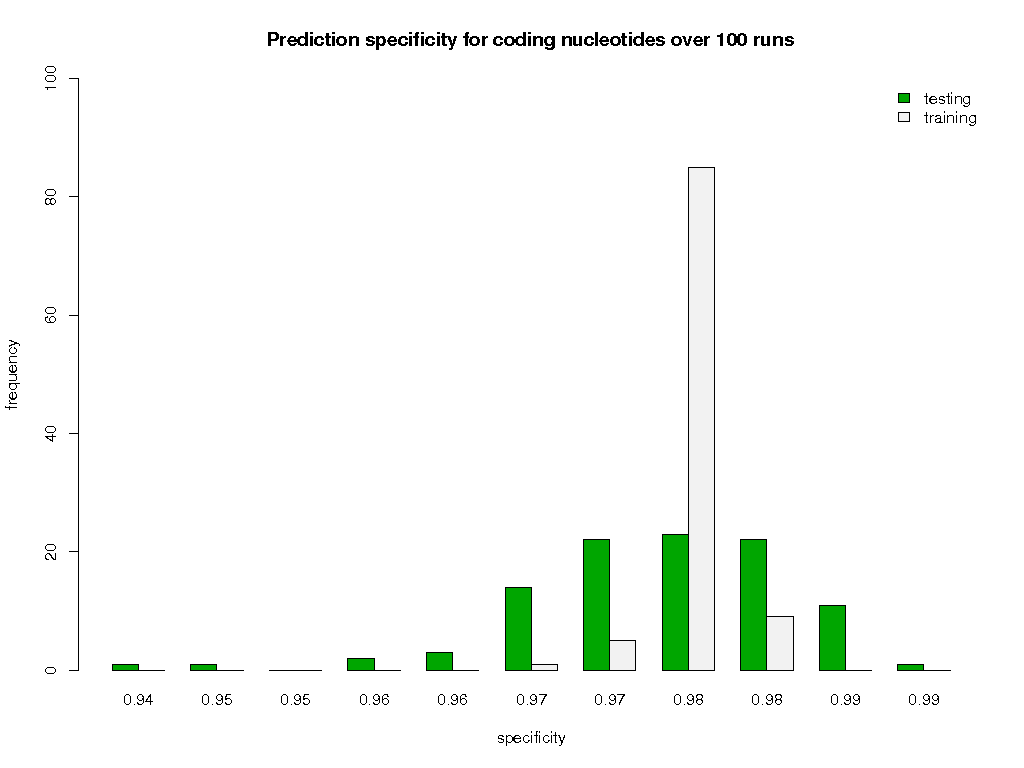
\includegraphics[scale=0.42]{pics/codingNucleotides_spec.png}
	\caption[Prediction specificity for coding nucleotides over 100 runs]{
	\textbf{Prediction specificity for coding nucleotides over 100 runs.}
	something}
	\end{center}
	\label{fig:codingNucleotides_spec}
\end{figure}

\begin{figure}[ht]
	\begin{center}
		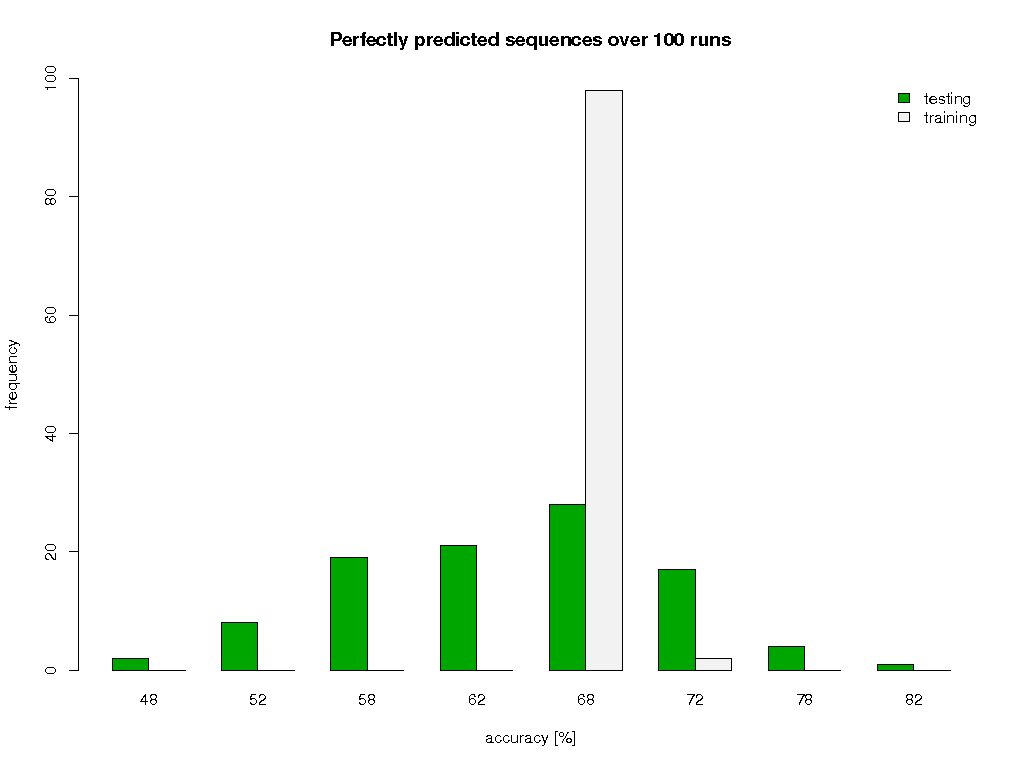
\includegraphics[scale=0.42]{pics/perfect2.png}
	\caption[Perfectly predicted sequences over 100 runs]{
	\textbf{Perfectly predicted sequences over 100 runs.}
	something}
	\end{center}
	\label{fig:perfect2}
\end{figure}

\begin{figure}[ht]
	\begin{center}
		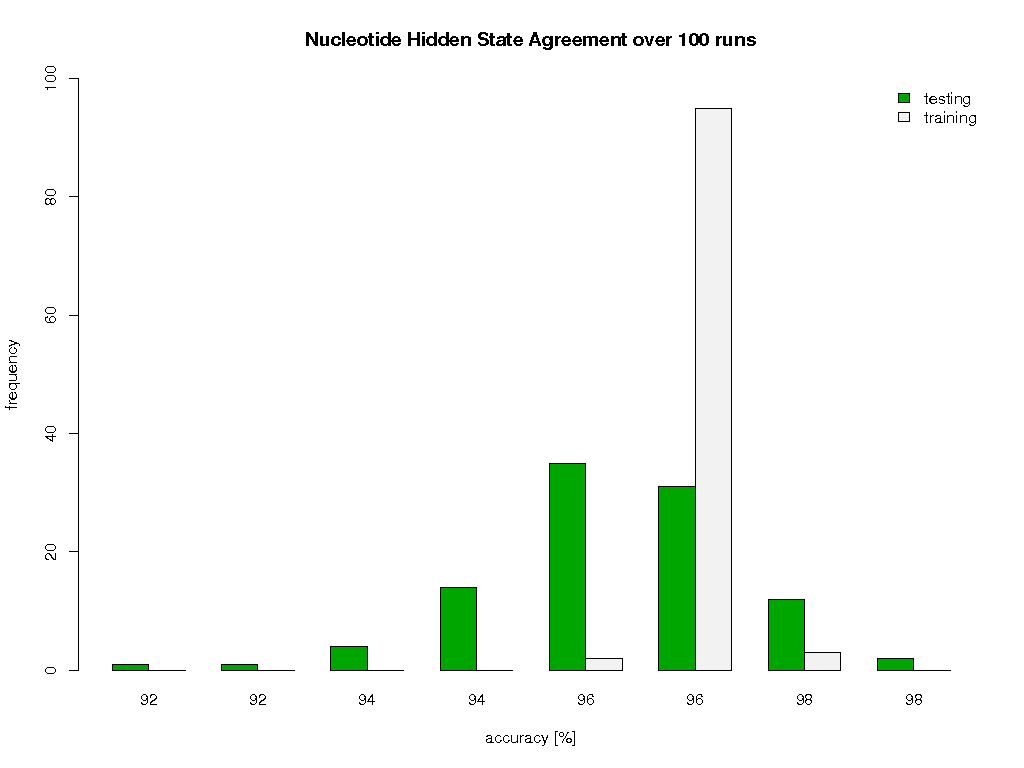
\includegraphics[scale=0.42]{pics/agree2.png}
	\caption[Nucleotide Hidden State Agreement over 100 runs]{
	\textbf{Nucleotide Hidden State Agreement over 100 runs.}
	something}
	\end{center}
	\label{fig:agree2}
\end{figure}

\paragraph{Conrad-local}
\paragraph{Conrad-lsf}
\subsubsection{RepeatMasker}
RepeatMasker
(\htmladdnormallink{http://www.repeatmasker.org/}{http://www.repeatmasker.org/})
ist ein Open Source Projekt, das repetetive Elemente einer Sequenz
\enquote{maskiert}, um so Rauschen während ähnlichkeitsbasierter Suchen zu
unterdrücken.
Die Maskierung kann entweder durch das Ersetzten der betroffenen Sequenzen
durch \enquote{N}'s bzw. \enquote{X}'s oder auch durch Ändern der Basen zur
Kleinschreibweise erfolgen.
Letzteres wird beispielsweise von \textit{BLAST} erkannt, was zur Folge hat,
dass diese Sequenzabschnitte nicht in der Suche berücksichtigt werden.
Die ursprüngliche Sequenzinformation bleibt auf diese Weise	erhalten.

\paragraph{RepeatMasker-local}

\paragraph{RepeatMasker-lsf}

\subsection{Libraries}
Neben den Basisfunktionalitäten und den bereits erwähnten Steps
beinhaltet Anna noch verschiedene Bundles, die Klassen aus externen Libraries
bereitstellen:
\begin{description}
\item[bioutils] dieses Bundle bringt 
\end{description}
